\chapter{Evaluation Data Acquisition}
\section{Data Acquisition}
For measurement on the true surface topography of snake sheds, samples are stuck on glass plates using double face tape, the animal was pushed up below a hollowed plate letting the skin emerging from the top of the plate using an atomic force microscope (AFM). An AFM is a microscope that uses a tiny probe mounted on a cantilever to scan the surface of an object. The probe is extremely close tobut does not touch the surface. As the probe traverses the surface, attractive and repulsive forces arising between it and the atoms on the surface induce forces on the probe that bend the cantilever. The amount of bending is measured and recorded, providing a map of the atoms on the surface. Atomic force microscopes is a very high-resolution type of scanning probe microscopy, with demonstrated resolution on the order of fractions of a nanometer, more than 1000 times better than the optical diffraction limit.

\section{Diffraction Gratings}
An idealised grating like in figure $\ref{fig:lighthitsgrating}$ is made of a very large number of parallel, evenly spaced slits in an opaque sheet. Typically, it would have about 10,000 slits. In order to cause diffraction, the spacing between slits must be wider than the wavelength of the incoming light beam. Each slit in the grating acts as a quasi point light source from which light propagates in all directions. Figure $\ref{fig:spectometer}$ illustrates this behaviour for a monochromatic light source passing through a grating and shows that the the outgoing angle will be different from the incident angle. Hence, the diffracted light $\ref{diffractiondeff}$ is composed of the sum of interfering wave components emanating from each slit in the grating.

\begin{figure}[H]
  \centering
  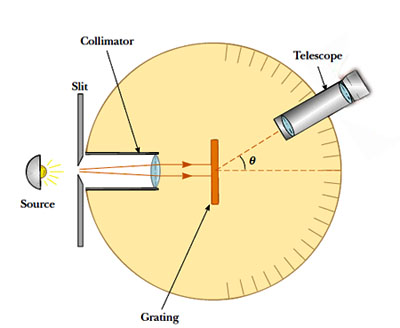
\includegraphics[scale=0.7]{evaluation/spectrometer.jpg}
  \caption{Spectometer: When a beam of monochromatic light passes through a grating placed in a spectrometer, images of the sources can be seen through the telescope at different angles.}
\label{fig:spectometer}
\end{figure}

Suppose monochromatic light is directed at the grating parallel to its axis as shown in figure $\ref{fig:spectometer}$. Let the distance between successive slits be equal $d$.

\begin{figure}[H]
  \centering
  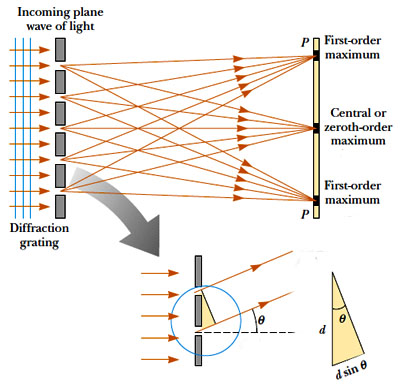
\includegraphics[scale=0.7]{evaluation/grating2.jpg}
  \caption{Light directed to parallel to grating:}
  \label{fig:lighthitsgrating}
\end{figure}

The diffraction pattern on the screen is the result of the combined effects of diffraction and interference. Each slit causes diffraction, and the diffracted beams in turn interfere with one another to produce the pattern. The path difference between waves from any two adjacent slits can be found by dropping a perpendicular line between the parallel waves. By geometry, this path difference is $d sin(\theta)$. If the path difference equals one wavelength or some integral multiple of a wavelength, waves from all slits will be in phase and a bright line will be observed at that point. Therefore, the condition for maxima in the interference pattern at the angle $\theta$ is: 

\begin{equation}
 d sin(\theta) = m \lambda 
\label{eq:simplegratingequation}
\end{equation}

where $m \in \mathds{N}_0$ is the order of diffraction.

Because $d$ is very small for a diffraction grating, a beam of monochromatic light passing through a diffraction grating is splitted into very narrow bright fringes at large angles $\theta$.

\begin{figure}[H]
  \centering
  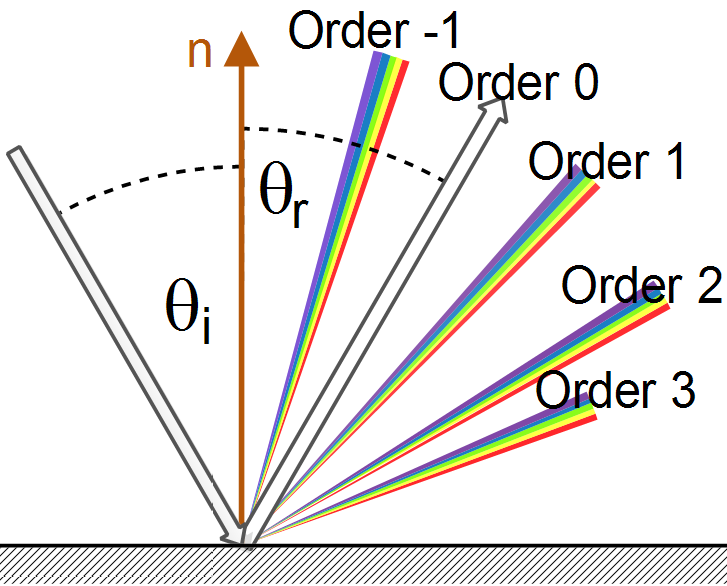
\includegraphics[scale=0.7]{evaluation/GratingSurface.png}
  \caption{Different Orders of diffraction}
\label{fig:gratingdiffractionorders}
\end{figure}

When a narrow beam of white light is directed at a diffraction grating along its axis, instead of a monochromatic bright fringe, a set of colored spectra are observed on both sides of the central white band as shown in figure $\ref{fig:gratingdiffractionorders}$.

\begin{figure}[H]
  \centering
  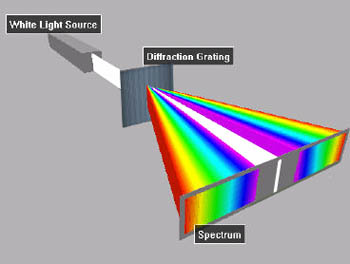
\includegraphics[scale=0.7]{evaluation/coloredspectrum.jpg}
  \caption{White Light beam causes coloured diffraction spectra}
  \label{fig:diffractionSpectrum}
\end{figure}

Since the angle $\theta$ increases with wavelength $\lambda$, red light, which has the longest wavelength, is diffracted through the largest angle. Similarly violet light has the shortest wavelength and is therefore diffracted the least. This relationship between angle and wavelength is illustrated in figure $\ref{fig:diffractionSpectrum}$. Thus, white light is split into its component colors from violet to red light. The spectrum is repeated in the different orders of diffraction, emphasizing certain colors differently, depending on their order of diffraction like shown in figure $\ref{fig:gratingdiffractionorders}$. Note that only the zero order spectrum is pure white.  
Figure $\ref{fig:nslitdiffractionintensity}$ shows the relative intensity resulting when a beam of light hits a diffraction grating for different number of periods. From the graph we recognise that the more slits a grating has, the sharper more slopes the function of intensity gets. This is similar like saying that, the more periods a grating has, the sharper the diffracted color spectrum gets like shown in figure $\ref{fig:diffractionslits}$. 

\begin{figure}[H]
  \centering
  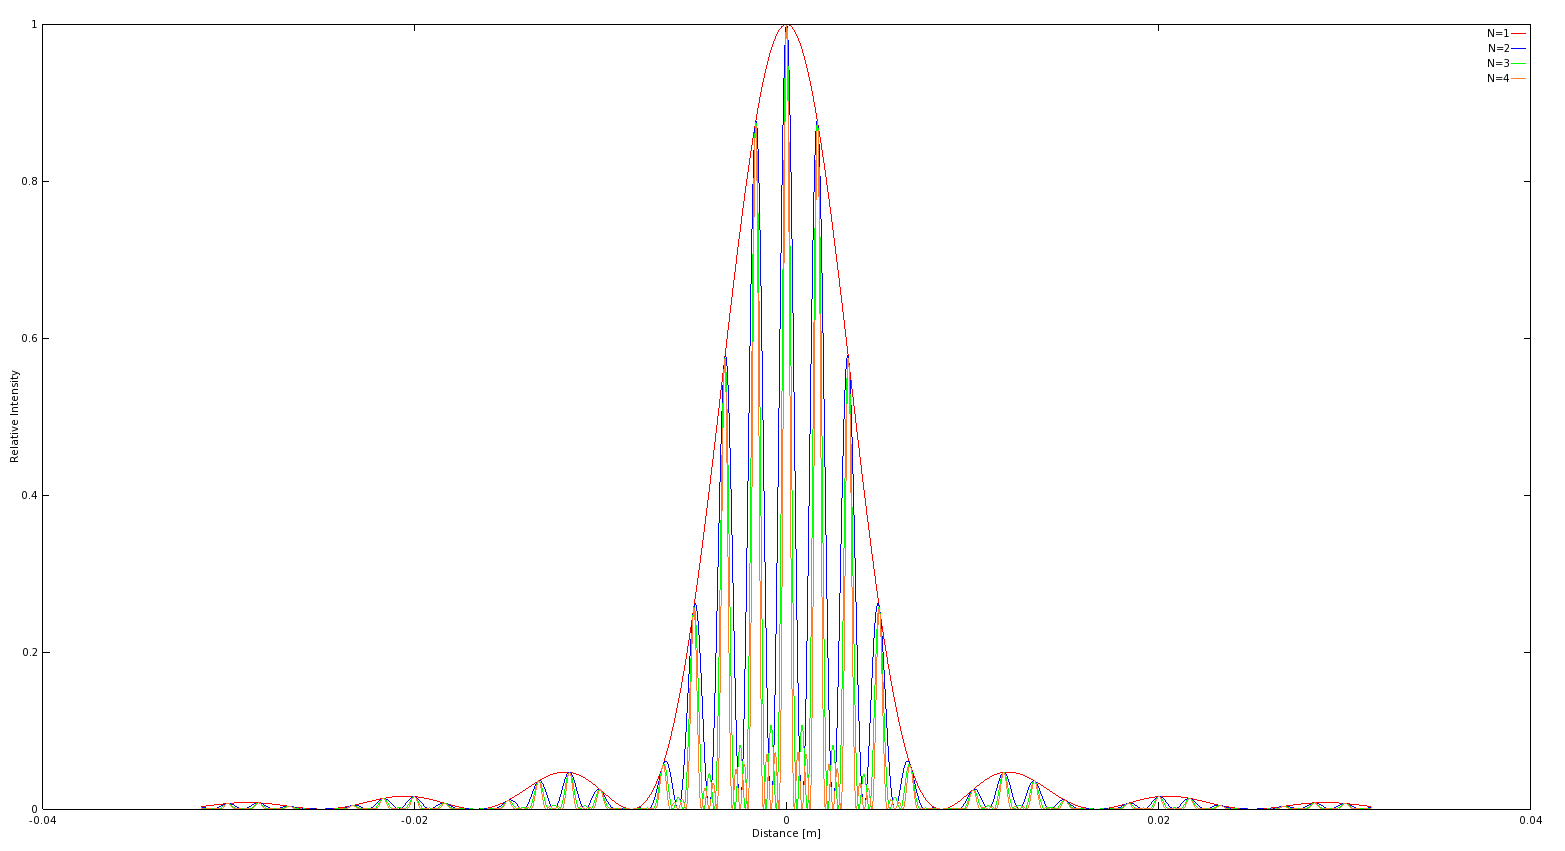
\includegraphics[scale=0.35]{evaluation/nslitdiffraction.png}
  \caption{Relative intensitiies of a diffracted beam of light at wavelength $\lambda=500nm$ on a grating for different number of periods $N$ width slit width of 30 microns and slit seperation of 0.15 mm each. The viewer is 0.5m apart from the grating.}
  \label{fig:nslitdiffractionintensity}
\end{figure}

\begin{figure}[H]
  \centering
  \subfigure[one slit]{
    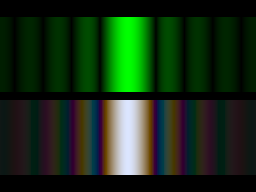
\includegraphics[scale=0.2]{evaluation/slits/spalt1.png}
    \label{fig:diffractionSlits1}
  }

~
  \subfigure[seven slits]{
    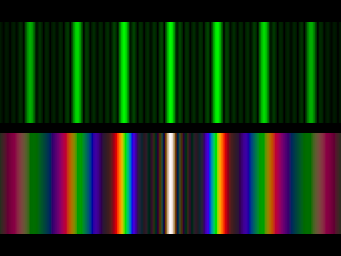
\includegraphics[scale=0.2]{evaluation/slits/spalt07.png}
    \label{fig:diffractionSlits7}
  }
  
  
  \caption{Difference of diffraction pattern between a monochromatic (top) and a white (bottom) light spectra for different number of slits.}
\label{fig:diffractionslits}
\end{figure}

\section{Evaluation}

\begin{figure}[H]
  \centering
  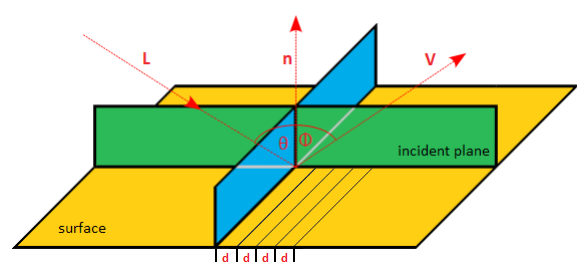
\includegraphics[scale=0.65]{evaluation/evalsetup.png}
  \caption{Experimental setup for evaluation: A light beam with direction $L$ hits the surface, representing a grating pattern with periodicity $d$, at the incident plane relative to the surface normal $n$ at angle $\theta$ and emerges at angle $\phi$ with direction $V$.}
  \label{fig:experimentalsetup}
\end{figure}

In order to check the physical reliability of our BRDF models, we applied them on a synthetic blazed grating, the Elaphe and Xenopeltis snake sheds and evaluated their response using the grating equation. This equation models the relationship between the grating spacing and the angles of the incident and diffracted beams of light. 

Figure $\ref{fig:experimentalsetup}$ illustrates the geometrical setup for our evaluation approach: A monochromatic beam of light with wavelength $\lambda$ hits a surface with periodicity $d$ at an angle $\theta$ relative to the normal $n$ along its incident plane. The beam emerges from the surface at the angle $\phi$. 

\begin{figure}[H]
  \centering
  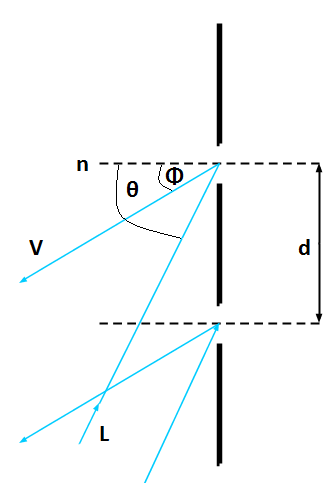
\includegraphics[scale=0.45]{evaluation/reflgrating.png}
  \caption{Reflecting grating: When the incident light direction is not parallel to its axis at the grating, there is another $sin(\phi)$ involved. See also the grating equation $\ref{eq:gratingeq}$.}
  \label{fig:reflgrating}
\end{figure}

The maximum in intensity is given by the grating equation derived from the equation $\ref{eq:simplegratingequation}$ following figure $\ref{fig:reflgrating}$: 

\begin{equation}
  sin(\theta) = sin(\phi) + \frac{m \lambda}{d}
\label{eq:gratingeq}
\end{equation}

In our evaluation we are interested in the zero order diffraction, i.e. m equals zero which corresponds to direct transmission or specular reflection in the case of a reflection grating. Within our evaluation we further assume that the incident light direction $w_i$ is given. In contrast the direction of the reflected wave $w_r$ is not given.
In Mathematics, a three dimensional direction vector is fully defined by two two angles, i.e. it can be represented by spherical coordinates with radius $r = 1$. By convention, we denote those two vectors by $\theta$ and $\phi$. Hence, $\theta_i$, $\phi_i$ and $\phi_r$ are given constants whereas $\theta_i$ is a free parameter for our evaluation simulation. Therefore, we are going to compare the maxima for peak viewing angle corresponding to each wavelength using data produced by our method against the maxima resulting by the grating equation.

\subsection{Precomputation}
Before being able to compare the output produced by our method by the grating equation, we have to discretise the wavelength space $\Lambda$ and the range $\Theta$ of our free parameter $\theta_i$. We also have to initially assign  $\theta_i$, $\phi_i$ and $\phi_r$. For our experiments we choose the following initial setup: $\theta_i = 75$ $\phi_i = 0$ $\phi_r = 180$ degree.
Further we discretise the lambda space $\Lambda = \{\lambda | \lambda = \lambda_{min} + k\lambda_{step}, k \in \{0,..,C-1\}\}$ where $\lambda_{step} = \frac{\lambda_{max}-\lambda_{min}}{C-1}$ and $C$ is the discretisation level of the lambda space, in our scenario $C = 42$. We similarly discretise the angle space by predefining an minimal and maximal angle boundary and $ceil(angMax - angMin) / angInc$ is the number of angles. 
We are going implement a similar algorithm as the diffraction fragment shader algorithme on the grid $[\Lambda, \Theta]$ and will store its spectral response in a matrix $R = \{response(\lambda_i, \theta_{r}^{j}) | i index(\Lambda), j index(\Theta)\}$. We also have evaluated our other shaders, mentioned within the discussion of the derivation and implementation chapters.

\subsection{Data evaluation}

\begin{algorithm}[H]
\caption{Evaluation: lambda thetar graph}
\label{alg:evalmatlab}
\begin{lstlisting}
% load all variables computed in java
lInc = (lMax - lMin)./(lambdaCnt-1);
lambda = lMin + lInc*(-1+[1:lambdaCnt]);
[maxC maxI] = max(response.');
viewAngForMax = angMin + angInc * (maxI-1);
plot(lambda, viewAngForMax,'-r');s

for thetaI=baseAngle-eps:0.5:baseAngle+eps,
	% grating equation
	thetaV = asin(lambda./dPeriod - sin(thetaI*pi()/180))*180/pi();
	if(thetaI==75)
		plot(lambda, thetaV,'+ b');
	else
		plot(lambda, thetaV,'. g');
	end
end

\end{lstlisting}
\end{algorithm}

\begin{figure}[H]
  \centering
  \subfigure[Blaze grating]{
    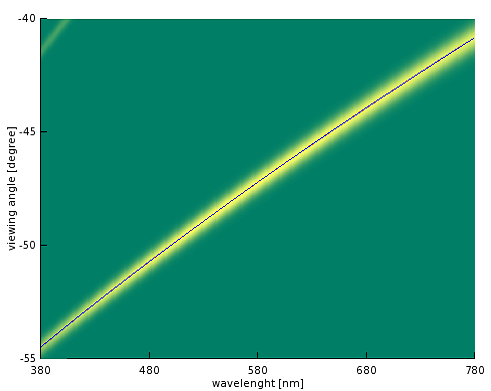
\includegraphics[scale=0.42]{evaluation/blazeHR.png}
    \label{fig:blazeval}
  }
~
  \subfigure[Xenopeltis]{
    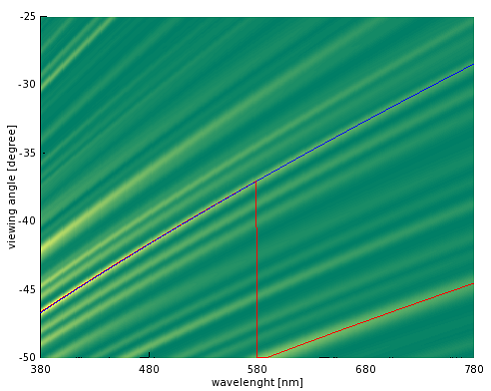
\includegraphics[scale=0.42]{evaluation/XenoHR.png}
    \label{fig:xenopeltiseval}
  }
~
\subfigure[Elaphe]{
  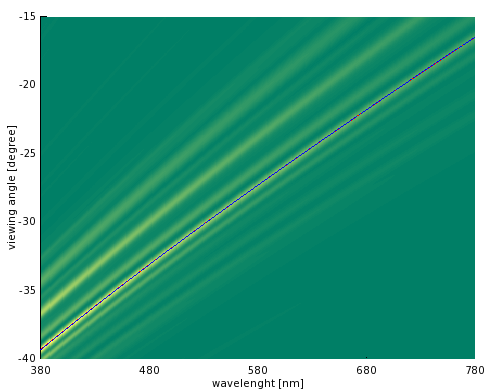
\includegraphics[scale=0.75]{evaluation/ElapheHR.png}
  \label{fig:elapheeval}
}

  \caption{Reflectance obtained by using the shading approach described in algorithm $\ref{alg:fragmentshaderall}$ simulating a BRDF which models the effect of diffraction at different viewing angles over the spectrum of visible light.}

\label{fig:evaluationdiffshaderalllambda}
\end{figure}

Figure $\ref{fig:evaluationdiffshaderalllambda}$ shows fits of order one diffraction angles of idealized periodic structures using illumination angle $\theta = 75$ degrees. The graphs $\ref{fig:elapheeval}$ and $\ref{fig:elapheeval}$ in figure $\ref{fig:evaluationdiffshaderalllambda}$ show reflectance of different nano-scaled structures computed by the uniform wavelength sampling fragment shader described as in algorithm $\ref{alg:fragmentshaderall}$. Higher values are in yellow, lower values in green. Viewing angles for peak reflectances of the nanostructues at each wavelength (red curve) and diffraction angles for an idealized periodic structure with a certain periodicity $d$ according to the grating equation $\ref{eq:gratingeq}$.

For each of the graphs we determine the vieweing angles with peak reflectance for various wavelengths and then plot this peak viewing angles against their wavelength as solid red curves. This red curve closely matches the blue curve representing the grating equation with the value of a edstimated from the peak view angles, listed in external source.


since blazed grating is synthetic we use its exact periodicity to plot the blue curve instead of estimating it. xeno evaluated just along the direction for the finger like structures.

the red and blue curve are closely overlapping in our figures $\ref{fig:blazeval}$ and $\ref{fig:elapheeval}$. For blaze and elaphe there is only diffraction along only along one direction perceivable.

for xeno its interesting to see that the red curve for the peak viewing angle toggles between two ridges correspinding to two different periodicities. this happens because there are multiple sub regions of the nanostructure whith slithly different orientations and periodicit. Each sub region carves out a different yellowish ridge. depending on the viewing agnle, reflectance due to one such subregion can be higher than from the others.




subvariants: sample whole lambda space, just a few lambdas, pq approach.
discussion
